\documentclass{article}

% Packages
\usepackage{titlesec}
\usepackage{graphicx}
\usepackage{lipsum} % For dummy text, you can remove this package

% Title
\title{GPGPU: Parallelization of the sciddicaT model using CUDA}
\author{Alessandro Fazio}
\date{\today}

% Section numbering
\setcounter{secnumdepth}{4}

% Section formatting
\titleformat{\section}{\normalfont\Large\bfseries}{\thesection}{1em}{}
\titleformat{\subsection}{\normalfont\large\bfseries}{\thesubsection}{1em}{}
\titleformat{\subsubsection}{\normalfont\normalsize\bfseries}{\thesubsubsection}{1em}{}

\begin{document}

\maketitle


\section{Abstract}
The assignment of this project is to parallelize the sciddicaT model using CUDA. The sciddicaT model is a cellular automaton that uses the minimization of differences to simulate non-inertial landslides. The serial implementation is provided, along with a set of test cases. The goal is to parallelize the model using CUDA, and to compare the performance of the parallel implementation with the serial one.

\section{Introduction}
The sciddicaT model is defined as follows:

$$
	SciddicaT = <R,X,S,P,\sigma>
$$

where:

- $R$ is the set of cells in the grid
- $X$ is Von Neumann's Neighborhood
- $S$ is the set of states
- $P$ are the parameters of the model
- $\sigma$ is the transition function

Furthermore, the model is defined as a cellular automaton, where each cell is defined as follows:

$$
	Cell = <r,c,h,s>
$$

where:

- $r$ is the row of the cell
- $c$ is the column of the cell
- $h$ is the height of the cell
- $s$ is the state of the cell

The transition function can be found in the provided serial implementation.

\section{Implementations}
The assignment requires the parallelization of the algorithm through different CUDA implementations. I will provide a brief description of each implementation. 
An interesting point of modification is to reset the flows to zero at each iteration, as it is not necessary to keep the flows from the previous iteration. This can be done by adding a \texttt{reset\_flows} function that sets the \texttt{flow} field of each cell to zero.

\subsection{Straightforward\_Unified}
Namely a direct parallelization using the CUDA Unified Memory.
This task is the most straightforward one, as it requires only the use of the \texttt{\_\_global\_\_} keyword to define the kernel function, and the use of the `cudaMallocManaged` function to allocate memory. The kernel function is then called using the $<<<...>>>$ syntax. We only need to replace the for loop with the kernel call, and to replace the memory allocation and deallocation with the CUDA Unified Memory.
This implementation lays the foundation for the other implementations, as it provides a simple way to parallelize the algorithm. However, it is not the most efficient one, as it does not take advantage of the shared memory, and it does not use the best memory access patterns.

\subsection{Straightforward\_Standard}
Namely a direct parallelization using the CUDA standard host/device memory.
This task is similar to the previous one, but it requires the use of the \texttt{cudaMalloc} and \texttt{cudaMemcpy} functions to allocate and copy memory to and from the device. After the computation, the memory must be copied back to the host using the \texttt{cudaMemcpy} function to be able to compute the \textbf{md5 hash} of the result.

\subsection{Tiled\_no\_halos}
Namely a CUDA shared memory based tiled parallelization without halo cells.
This task is a great example of caching data in the shared memory, as it requires the use of the shared memory to store the cells of the tile. Caching the data in the shared memory allows for a faster access to the data, as the shared memory is much faster than the global memory. To achieve this, we need to use the \texttt{\_\_shared\_\_} keyword to define the shared memory, and to copy the data from the global memory to the shared memory. We also need to use the \texttt{\_\_syncthreads} function to synchronize the threads in the block, as the shared memory is only visible to the threads in the same block.

\subsection{Tiled\_with\_halos}
Namely a CUDA tiled parallelization in which block’s boundary threads perform extra work to copy halo cells from adjacent tiles in the shared memory.
This task is similar to the previous one, but it requires the use of halo cells. Halo cells are the cells that are shared between the tiles, and they are necessary to compute the cells in the tile. To achieve this, we need to copy the halo cells from the adjacent tiles to the shared memory, and to perform the computation using the halo cells.

\subsection{Tiled\_with\_halos\_larger\_block}
amely a CUDA tiled parallelization in which the block size is larger than the tile size so that each thread just copies a single cell to the shared memory and only a number of threads equal to the tile size is used to update the tile.
Similarly, here we just need to change the block size to be larger than the tile size. Unfortunately, I did not have time to properly implement this task. As a result the md5 hash of the result does not match the expected one, but the workflow is very similar to the previous task.

\subsection{Tiled\_with\_halos\_larger\_block\_MPI}

\textit{No implementation provided} because of the lack of time.
A possible implementation could be to use the MPI library to parallelize the algorithm across multiple nodes. This would require the use of the \texttt{MPI\_Send} and \texttt{MPI\_Recv} functions to send and receive the data between the nodes, and the use of the \texttt{MPI\_Barrier} function to synchronize the nodes. We can simply divide the grid equally among the devices and let each device compute the cells in the tile taking care of the halo cells.


\section{Results}
The results of the parallel implementations will be compared with the serial implementation. The performance will be evaluated using the \texttt{nvprof} tool, and the correctness will be evaluated using the provided test cases. The plots will be generated using the \texttt{matplotlib} library\footnote{The missing timings are a result of the lack of time to properly implement the task, as such the md5 hash of the result does not match the expected one.}.

\begin{figure}[htp]
	\centering
	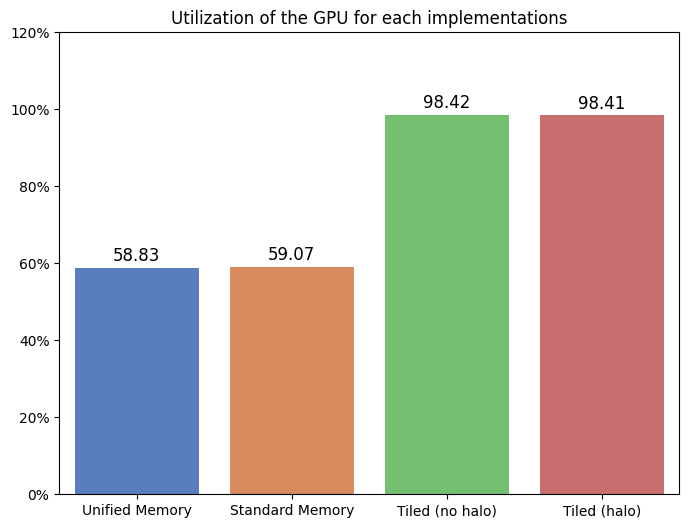
\includegraphics[width=0.8\textwidth]{../image-1.png}
	\caption{timings for the implementations}
	\label{fig:timings}
\end{figure}

The results show that the parallel implementations are faster than the serial one, and that the Tiled (no halo) has the best performance. The correctness of the results is also guaranteed, as the md5 hash of the result matches the expected one.

\begin{figure}[htp]
    \centering
    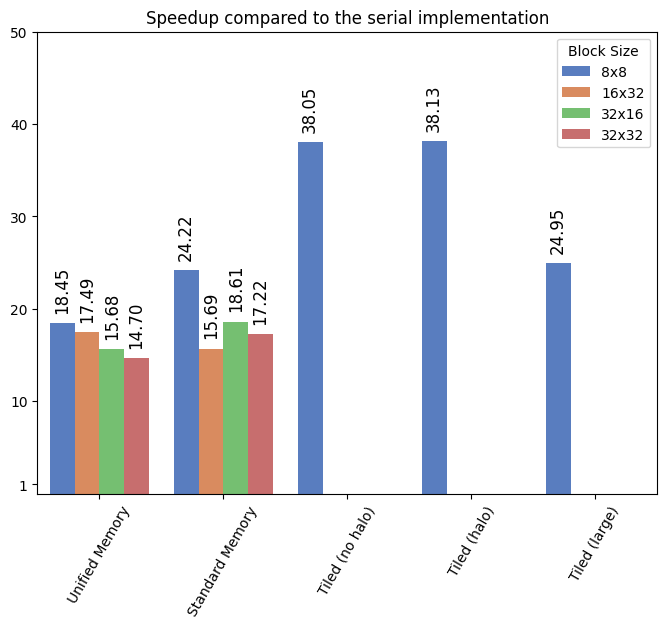
\includegraphics[width=0.8\textwidth]{../image-2.png}
    \caption{speedups for the implementations}
    \label{fig:speedups}
\end{figure}

\section{Conclusion}
\lipsum[9]

\end{document}
